%%%%%%%%%%%%%%%%%%%%%%%%%%%%%%%%%%%%%%%%%%%%%%%%%%%%%%%%%%%%%%%%%%%%%%%%%%%

\documentclass{standalone}

\usepackage{mathptmx}
\usepackage{tikz}
\usetikzlibrary{external}
\tikzexternalize{robot-path-square-triangle}

%% We default to Times.
\renewcommand{\rmdefault}{ptm}
\renewcommand{\ttdefault}{pcr}
%% Enable Times/Palatino main text font.
\normalfont\selectfont

\newcommand{\comma}{,\,}
\newcommand{\tuple}[2]{(#1\comma #2)}

%% A tick on the x-axis.
%%
%% #1 -- A point on the x-axis.
\newcommand{\xtick}[1]{%%
  \draw[tickStyle] (#1,\tickdx) -- (#1,-\tickdx);
  \node at (#1,-\tickdx) [below] {$#1$};
}

%% A tick on the y-axis.
%%
%% #1 -- A point on the y-axis.
\newcommand{\ytick}[1]{%%
  \draw[tickStyle] (-\tickdx,#1) -- (\tickdx,#1);
  \node at (-\tickdx,#1) [left] {$#1$};
}

%% The Cartesian coordinate system.
\newcommand{\cartesianCoordinate}{%%
  %% The x-axis.
  \draw[axisStyle] (xstart) -- (xend);
  \foreach \x in {-4,-3,-2,-1,1,2,3,4}{
    \xtick{\x}
  };
  \node at (xend) [right] {$x$};
  %% The y-axis.
  \draw[axisStyle] (ystart) -- (yend);
  \foreach \y in {1,2,3,4}{
    \ytick{\y}
  };
  \node at (yend) [above] {$y$};
}

%% A square path on the Cartesian plane.  The lower-left point is
%% assumed to be the origin.
%%
%% #1 -- The x-coordinate of the upper-right point.
%% #2 -- The y-coordinate of the upper-right point.
%% #3 -- Label the point with this name.
%% #4 -- Where to place the label relative to the point.
\newcommand{\squarePath}[4]{%%
  \draw[redStyle] (origin) rectangle (#1,#2);
  \node[nodeStyle] at (#1,#2) {};
  \node at (#1,#2) [#4] {$#3$};
  \node[nodeStyle] at (#1,0) {};
  \node[nodeStyle] at (0,#2) {};
}

%% A triangle path on the Cartesian plane.  One of the points is the
%% origin.
%%
%% #1 -- The x-coordinate of the point.
%% #2 -- The y-coordinate of the point.
%% #3 -- Label the point with this name.
%% #4 -- Where to place the label relative to the point.
\newcommand{\trianglePath}[4]{%%
  \draw[redStyle] (origin) -- (-3,3) -- (-3,0) -- cycle;
  \node[nodeStyle] at (#1,#2) {};
  \node at (#1,#2) [#4] {$#3$};
  \node[nodeStyle] at (#1,0) {};
  \node[nodeStyle] at (0,0) {};
}

%% The Cartesian coordinate system.

\begin{document}

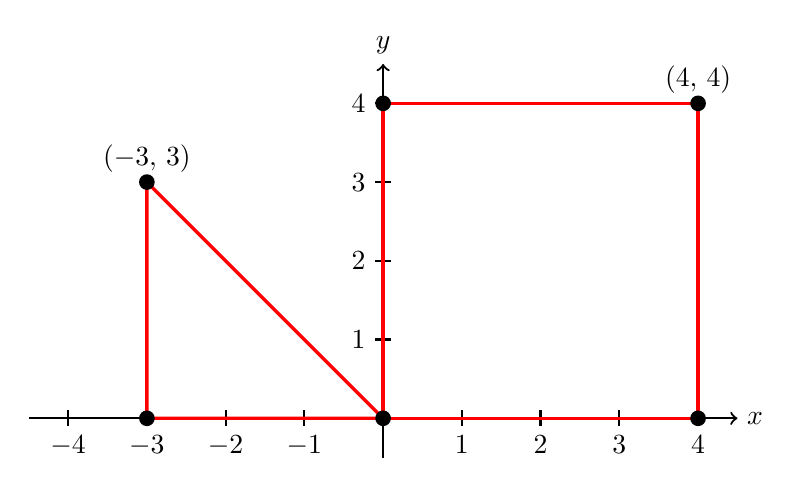
\begin{tikzpicture}[%%
  axisStyle/.style={->,thick},%%
  redStyle/.style={-,red,very thick},%%
  nodeStyle/.style={circle,inner sep=2pt,fill=black,black},%%
  tickStyle/.style={-,thick}
]
%%
%%
\pgfmathsetmacro{\tickdx}{0.1}
\pgfmathsetmacro{\xhigh}{4.5}
\pgfmathsetmacro{\xlow}{-4.5}
\pgfmathsetmacro{\yhigh}{4.5}
\pgfmathsetmacro{\ylow}{-0.5}
\coordinate (origin) at (0,0);
\coordinate (xend) at (\xhigh,0);
\coordinate (xstart) at (\xlow,0);
\coordinate (yend) at (0,\yhigh);
\coordinate (ystart) at (0,\ylow);
%%
%% The Cartesian coordinate system.
\cartesianCoordinate
%%
%% Paths on the Cartesian plane.
%% Square path with point (4,4).
\squarePath{4}{4}{\tuple{4}{4}}{above}
%% Triangle path with point (-3,3).
\trianglePath{-3}{3}{\tuple{-3}{3}}{above}
\end{tikzpicture}

\end{document}
